0A\appendix
\chapter{Basics of Statistical Physics}
The proceeding derivations follow Cardy~\cite{cardy} and Domb~\cite{domb}.
\section{Measurements as Averages}\label{sec:measurements-as-averages}
Suppose we want to test whether our theory, the Ising model, lines up
with experimental results: what are the kinds of predictions we can
make? Our first attempt might be to measure the system's
magnetization, rather appropriate as this is the defining
characteristic of ``magnets.'' Before we do, however, let us be more
precise. What is a measurement, specifically for magnetization? The
magnetization, $M$, of any one microstate, $\bs$ is simply the sum of
the orientations of all spins, $s_i\in\bs$ in a given state:%
\begin{equation}%
  M(\bs)=\sum_{i} s_i,
  \label{eq:magnetization}
\end{equation}%

Generally, the microscopic state of a system is changing rapidly, and
the system will explore many different microstates over human
time-scales. Our measuring devices have finite resolution in time, so,
in a laboratory, we cannot perform sums over individual microstates. A
measurement becomes the average over the microstates visited during
the measurement period, weighted by the time spent in each state. In
statistical physics, we often work in the limit that the update time
goes to zero compared to the time of measurement. In this light, the
notion of a probability of a microstate is also the fraction of time
the system spends in that microstate over an infinite duration. Our
measurement outcome, $\mc{M}$, is an expectation value,
$\expect{M(\bs)}$, the average over the set of all microstates,
$\mcS=\{\bs\}$, weighted by the amount of time spent in each state,
$P(s)$:%p
% TODO: BETTER NOTATION (\bs conflicts with E(\bs)
\begin{equation}%
  \mc{M}=\expect{M(\bs)}=\sum_{\bs\in\{\bs\}}P(\bs)M(\bs).
  \label{eq:magnetization-expectation}
\end{equation}%
The same holds for any measurable quantity. Given some function of a
microstate, $A(\bs)$, the macroscopic value it corresponds to is its
expectation value over all microstates, $\expect{A(\bs)}$. Common
examples (not restricted to the Ising model) include $E(\bs)$, the
energy, $P(\bs)$, the pressure, and $V(\bs)$, the volume. If we can
find a probability measure over microstates, we can use the above to
calculate any macroparameter we choose.

\section{Thermal Equilibrium and the Second Law of
  Thermodynamics}\label{sec:delta-s-delta-e}
Consider the first law of thermodynamics (differential form with only
one kind of particle):%
\begin{equation}%
  dE=TdS-PdV+\mu dN,
\end{equation}%
where $E$ is the energy, $T$ the temperature, $P$ the pressure, $V$
the volume, $\mu$ the chemical potential, and $N$ the number of
particles.

For the canonical ensemble (our example), $dV$ and $dN$ are $0$.
Then, this reduces to:
\begin{equation}%
  \frac{1}{T}dE=dS.
\end{equation}%

From \fref{eq:boltzmann-entropy-difference}, we have
$\Delta S=S_{\br}(\bs)-S_{\br}(\bs')$.  If the reservoir is much
larger than $\bs$, this is a tiny difference, so
$\Delta S \approx dS$.  Then, we get
$\Delta S \approx \frac{1}{T}(dE)$. Note that this requires the
reservoir and system to have the same temperature (i.e., to be in
thermal equilibrium, $T_{\br}=T_{\bs}$).  We can use the same
approximation to expand this out:
$dE\approx E_{\br}(\bs)-E_{\br}(\bs')=\Delta E$.  We end up
with~\fref{eq:boltzmann-energy-difference}.

Note that in the thermodynamic limit,
$\abs{\bs}, \abs{br}\rightarrow \infty$ while maintaining the
inequality $1\ll\abs{\bs}\ll\abs{\br}$, these statements are precise
(this is simply the central limit theorem).

\section{Observables as Derivatives of the Partition
  Function}\label{sec:Z-to-macros}
Let us define the free energy, $F=-\frac{1}{\b}\ln Z$, where $\b=k T$,
the so-called thermodynamic beta. Consider an energy function with a
dependence on parameter $A$ according to:%
\begin{equation}%
  E(\bs)=E_0(\bs)+\l A(\bs)
\end{equation}%

Then, $\expect{A}=\partial_\l F$ The derivation proceeds as:
\begin{align}%
  \expect{A(\bs)}&=\partial_\l \left( -\frac{1}{\b}\ln Z\right) \label{eq:expectation-as-derivative}\\
                 &=-\frac{1}{\b Z}\partial_\l Z\\
                 &=-\frac{1}{\b Z}\sum_{\bs} e^{-\b E(\bs)}\partial_\l\left(-\b E(\bs)\right) \\
                 &= \frac{1}{\b Z}\sum_{\bs} e^{-\b E(\bs)}\left(\b A(\bs) \right) \\
                 &= \sum_{\bs} \frac{e^{-\b E(\bs)}}{Z} A(\bs) \\
                 &= \sum_{\bs} P(\bs) A(\bs).
\end{align}%

Consider an example, taking the Ising Hamiltonian
(\ref{eq:ising-energy}):
\begin{align}%
  \partial_B \left(-\log Z\right)&=-\frac{1}{Z}\sum_{\bs}\partial_Be^{-B \sum_i s_i - J \sum_{\expect{i,j}} s_i s_j}\\
                                 &=-\sum_{\bs}\frac{e^{-E(\bs)}}{Z} (-\sum_i s_i)\\
                                 &=\sum_{\bs}P(\bs)M(\bs) \\
                                 &=\expect{M(\bs)}.\label{eq:magnetization-as-derivative}
\end{align}%

Two others:
\begin{align}%
  \chi&=\partial_B \mc{M}=\partial_B^2F\\
  E&=\partial_\b F.
\end{align}

\chapter{Scaling and Renormalization}
\section{Finite-Size Scaling Analysis}\label{sec:finite-size-scaling}\
This section follows~\cite{fssa}. In our theoretic discussion, we have typically considered infinite
lattices: for a fixed lattice size $L$, we have let the microscopic
size $a$ (the lattice width) go to zero. Then, the dimensionless
$N=L/a$ (the number of lattice sites in a given dimension) diverges;
this is the classical thermodynamic limit.  Of course, truly physical
systems are finite with correspondingly non-singular partition
functions. For any such systems, there can be no divergences. An
important concern is, then, determining under which conditions we can
treat our systems as infinite and under which conditions finite-size
effects have a non-neglibile effect.

An important tool we use to study critical systems is MCMC
simulations: here, we quickly run into computational limits on the
sizes of lattices we can simulate. Especially for MCMC techniques, the
role of finite-size scaling is crucial.

Consider a $d$-dimensional Ising model infinite in all directions. If
we were to decrease $N$ of one dimension to some finite value, the
system's critical behavior begins to be dominated by a $d-1$
dimensional critical point. This is an example of crossing-over
behavior. By controlling some relevant parameter we change the
effective dimensionality of our system and navigate between different
critical points.

An example of this finite-size behavior is that of the correlation
length, $\xi$. It will no longer diverge and depending on the boundary
conditions will experience a peak at either above or below the infinte
critical point. For cyclical boundary conditions, the effective
critical temperature will increase, as the system is more ordered with
more paths between spins. For zero-field boundary conditions, the
temperature will decrease as there less paths between spins.

We have seen from \fref{tab:crit-exponents}, that diverging quantities
$A(t,N^{-1}=0)$ scale as $\abs{t-t_c}^{-\zeta}$ for some critical
exponent $\zeta$. In the large $N$-limit, we expect that the system
will continue to behave as such, provided that $N$ is much greater
than the system's characteristic length scale, the correlation length,
$\xi\sim \abs{t-t_c}^{-\nu}$. This amounts to%
\begin{equation}%
  A(t, N^{-1})\sim \abs{t-t_c}^{-\zeta}\sim \xi^{\zeta/\nu}\tab (N \gg \xi, t\rightarrow t_c).
\end{equation}%
The system's geometry will act as a cutoff: rather than diverge, now,
as $\xi \rightarrow N$, $A$ will behave as%
\begin{equation}%
  A(t,N^{-1})\sim N^{\zeta/\nu}\tab (N \ll \xi, t\rightarrow t_c).
\end{equation}%

Together, these considerations give rise to the finite-scaling
ansatz:
\begin{equation}%
  A(t,N^{-1})\sim \xi^{\zeta/\nu} \phi((N\xi)^{-1})\tab (N^{-1}\rightarrow 0, t\rightarrow t_c),
\end{equation}%
where
\begin{equation}%
  \phi(x)\{
  \begin{cases}
    = \text{const.} &\text{for } \abs{x}\gg 1 \\
    \sim x^{\zeta/\nu} &\text{for } \abs{x}\rightarrow 0\\
  \end{cases}.
\end{equation}%
$phi(x)$ is a scaling function that controls the finite-size
effects. By convention, we choose the scaling function
$\tilde{\phi}(x)=x^{-\zeta}\phi(x^\nu)$. Then, we get that%
\begin{equation}%
  A(t,L) = L^{\zeta/\nu} \tilde{\phi}\left(L^{1/\nu} (t - t_c)\right), \tab (L \rightarrow \infty, t \rightarrow t_c),
\end{equation}%
with
\begin{equation}%
  \tilde{\phi}(x)
  \begin{cases}{}
    = \text{const.} & \text{for } x \to 0\tab  (L \ll \xi), \\
    \sim L^{-\zeta/\nu} (\varrho - \varrho_c)^{-\zeta} & \text{for }
    |x| \gg 1
    \tab (L \gg \xi).\\
  \end{cases}
\end{equation}.%
This is valuable because it allows us to plot
experimental data $a_{exp.}(t,L)$ collected at some temperature and lattice
size, on a single curve:%
\begin{equation}%
  \tilde{\phi(L^{1/\nu}(t-t_c))}=L^{-\zeta/\nu}A(t,L)
\end{equation}.%
Plotting $L^{1/\nu}(t-t_c)$ against $L^{-\zeta/\nu}A(t,L)|_{a_{exp.}(t,L)}$, our experimental data will ``collapse'' onto a single line.
In practice, it is enough to consider only the effective critical temperature
at different length scales. Plotting this against $\log L$, the points should
fall onto a single line with slope $\nu$.

\section{Scaling Rules for the
  Free-Energy}\label{sec:free-energy-scaling}
In this section, we will derive a transformation rule for the free
energy. From \fref{sec:Z-to-macros}, we know that we can use this
transformation rule to determine our critical exponents of interest.

Starting with~\ref{eq:rg-transformation-general}, we can intuit that
the free energy will take a form similar to:%
\begin{equation}
  f(\{K\})=g(\{K\})+ b^{-d}f(\{K'\}).
\end{equation}
we expect a function similar to our starting point but of the updated
coupling $f(\{K'\})$ and where we have rescaled the system by (for
example, a block-size) $b$. For $d$ dimensions, we rescale in each
direction. Furthermore, we could have some (analytic) function of our
coupling at a given instance, $g(\{K\})$.

The free energy of new system is equal to that of the original system
with some rescaling, plus the addition of a constant term. Note that
this is an inhomogenous transformation. However, for \textit{singular}
behavior (near the critical point), we only care about the second
term. $g()$ originates from summing over short degrees of freedom, and
it should be an analytic (non-divergent) function of $K_a$ even at
critical point.

Considering just the transformation rule for the singular part:
\begin{equation}
  f_s(\{K\})=b^{-d}f_s(\{K'\}).\label{eq:f-singular-transformation}
\end{equation}

We use our knowledge that there are are only two relevant scaling
variables, $u_t$ and $u_h$ (for the interested reader, we refer to
Cardy~\cite{cardy}). These possess important symmetries: $u_t$
corresponds to the even subspace of couplings (invariant a collective
sign-flip $\bs\rightarrow -\bs$), and $u_h$ to the odd subspace
(equivariant with the collective sign-flip). Let us reexpress the
above equation in terms of our scaling variables. First, we
Taylor-expand the scaling variables\footnote{This is valid since we
  have already limited ourselves to the immediate vicinity of the
  critical point.}. By these symmetry arguments, odd terms vanish from
$u_t$ and even terms from $u_h$. Looking at the formula for $u_i$, we
see they must vanish at $t=h=0$.
\begin{equation}
  u_t = \frac{t}{t_0} + O(t^2, h^2)\label{eq:u-t}
\end{equation}

\begin{equation}
  u_h = \frac{h}{h_0} + O(th)\label{eq:u-h}
\end{equation}

Near the critical point, we take these scaling variables to be
proportional to $h$ and $t$\footnote{In more complicated systems, and
  those with tricritical points, our relevant variables will not
  necessarily be directly proportional to the experimental variables
  (the knobs) we control.}. Combining our equations for the scaling
variables, (\ref{eq:u-t}) and (\ref{eq:u-h}), with the singular free
energy transformation:
\begin{equation}
  f_s(u_t,u_h)=b^{-d}f_s(b^{y_t}u_t,b^{y_h}u_h).
\end{equation}
If we repeat this transformation $n$ times, we get:
\begin{equation}%
  f_s(u_t,u_h)=b^{-nd}f_s(b^{ny_t}u_t, b^{y_h}u_h).\label{eq:f-repeated-transformations}
\end{equation}%

We now choose an arbitrary point $u_{t0}=\abs{b^{ny_t}u_t}$. This
constrains our $n$ to not be too large that the linear approximation
breaks down. Solving for $n$ we get:%
\begin{equation}
  n= \frac{1}{y_t} \log_b{(\abs{\frac{u_t}{u_{t0}}}^{-1})}.\label{eq:n-iterations}
\end{equation}

Plugging \fref{eq:n-iterations} into
\fref{eq:f-repeated-transformations}:
\begin{equation}
  f_s(u_t,u_h)=\abs{\frac{u_t}{u_{t0}}}^{\frac{d}{y_t}}f_s(\pm u_{t0}, u_h\abs{\frac{u_t}{u_{t0}}}^{-\frac{y_h}{y_t}}).
\end{equation}
Rewriting in terms of $t$ and $h$, where we incorporate $u_{t0}$ into
a new scale factor $t_0$ (i.e.,
$\frac{t}{t_0}\leftarrow \frac{t}{u_{t0}t_0}$):%
\begin{equation}
  f_s(t,h)= \abs{\frac{t}{t_0}}^{d/y_t}\Phi(\frac{\frac{h}{h_0}}{\abs{t/t_0}^{y_h/y_t}})
\end{equation}

We see that introducing this cutoff $u_{t0}$ has allowed us to express the
(approximately) a function of two variables, $f_s$, in terms of just
one variable in the \textit{scaling function} $\Phi$.

This scaling function may appear to include a $u_{t0}$ dependency, but
since the l.h.s\@. does not, this will cancel. These scaling functions
turn out to be universal, it only depends on the system through $t_0$
and $h_0$.

\section{The Correlation Length Critical
  Exponent}\label{sec:rg-correlation-length}
As an example of using free energy scaling to solve critical
exponents, let us attempt correlation length critical
exponent. Consider the two-point correlation function:%
\begin{equation}
  G(r_1-r_2,H)\equiv\langle s(r_1)s(r_2\rangle_H - \langle s(r_1)\rangle_H\langle s(r_2)\rangle_H
\end{equation}
Our first step will be to express this in terms of (derivatives of)
the free energy. We introduce a non-uniform magnetic field to our
Hamiltonian:
\begin{equation}
  H \rightarrow H - \sum_r h(r) s(r)
\end{equation}
and differentiate the free energy ($f=\ln{Z}$) twice:
\begin{align}
  G(r_1-r_2,H)= &\frac{\partial^2}{\partial h(r_1) \partial h(r_2)} \ln{Z(\{H\})}\rvert_{h(r)=0} \\
  =& \frac{\partial}{\partial h(r_1)}\left(-\frac{1}{Z}\sum_s s(r_2) e^{H(s)-\sum_r h(r) s(r)}\right)\rvert_{h=0} \\
  =& -\frac{1}{Z^2}\sum_{s'} s'(r_1) e^{H(s')-\sum_r h(r) s'(r)} \sum_s s(r_2) e^{H(s)-\sum_r h(r) s(r)}\\
                & - \frac{1}{Z}\sum_s s(r_1)s(r_2) e^{H(s)-\sum_r h(r) s(r)}\rvert_{h=0}\\
  =&-\left(\frac{1}{Z}\sum_{s'}s'(r_1)e^{H(s')}\right)\left(\frac{1}{Z}\sum_{s}s(r_1)e^{H(s)}\right) + \frac{1}{Z}\sum_s s(r_1)s(r_2)e^{H(s)} \\
  =&\langle s(r_1)s(r_2)\rangle_H - \langle s(r_1)\rangle_H\langle s(r_2)\rangle_H.
\end{align}

We suppose that $h(r)$ varies over scales much larger than block size
$ba$. Applying block renormalization we can effectively ignore the
varying of $h(r)$ within a given block. The, for a specified block, it
transforms as a uniform field would. The renormalization Hamiltonian
should be of the same form.
\begin{equation}
  H'(s')-\sum_{r'}h'(r')s'(r')
\end{equation}

Since RG preserves the partition function, we can write:
\begin{equation}
  \frac{\partial^2 \ln Z'(h')}{\partial h'(r_1') \partial h'(r_2')}=\frac{\partial^2 \ln Z(h)}{\partial h'(r_1') \partial h'(r_2')}
\end{equation}

Now the l.h.s.\ is just the correlation function of the RG system with
the new Hamiltonian. In terms of our original correlation function, we
have to rescale the distance by a factor b.
\begin{equation}
  G((r_1-r_2)/b, H')
\end{equation}

Onto the r.h.s. If we make a change in $h'(r')$, we will change
\textit{all} the spins contained in that block:
\begin{equation}
  \delta h(r_i)=b^{-y_h} \delta h'(r_1'),
\end{equation}
so this reduces to:
\begin{equation}
  b^{-2y_h}\langle (s_1^{(1)}+ s_2^{(1)}+\dots)(s_1^{(2)}+ s_2^{(2)}+\dots) \rangle_H.
\end{equation}
Each block contains $b^d$ spins, so expanding this gives us $b^{2d}$
2-point correlations. For our assumption that $r=\rvert r_1-r_2\rvert$
is large, each will give about the same result. For isotropic systems
(respecting rotational symmetries of the lattice), the correlation
function will only depend on distance between points, not on
orientation.

We end up with the transformation rule:%
\begin{equation}
  G((r_1-r_2)/b,H')=b^{2(d-y_h)}G(r_1-r_2,H).
\end{equation}

For simplicitly, we set $h=0$ and iterate $n$ times:
\begin{equation}
  G(r,t)=b^{-2(d-y_h)}G(r/b, b^{y_t}t)=b^{-2n(d-y_h)}G(r/b^n, b^{ny_t}t),
\end{equation}
stopping at some fixed point where $b^{ny_t}(t/t_0)=1$ (as we did for
the free energy in \fref{sec:free-energy-scaling}).  Then,
\begin{equation}
  n = -\frac{1}{y_t}\log_b(t/t_0),
\end{equation}
and plugging this in:
\begin{equation}
  G(r,t)=\abs{t/t_0}^{2(d-y_h)/y_t} \Psi\left(\frac{r}{\abs{t/t_0}^{-1/y_t}}\right).
\end{equation}
By definition, $G(r)\propto e^{-r/\xi}$ for $r\gg\xi$, near the
critical point (see argument in, for example,~\cite{cardy}).  From the
argument of the scaling function, $Psi$, we can identify that:
$\xi \propto \abs{t}^{-1/y_t}$.

Then,
\begin{equation}
  \nu=1/y_t
\end{equation}
\chapter{Basics of Information Theory}\label{sec:information-theory}
We begin with a random variable $x\in \mcX$, with the probability
distribution $P(x)$.  The \textit{information} in $x$ is:
\begin{equation}%
  I(x)=-\log_2 P(x).
\end{equation}%
To understand why this is more useful than $P(x)$, consider another
random variable $y\in \mcY$ with distribution $P(y)$. If the two
variables are independent ($P(x,y)=P(x)P(y)$), we get that their
information \textit{adds}:
\begin{equation}%
  I(x,y)=I(x)+I(y).
\end{equation}%
The logarithm is a powerful tool that converts multiplication (hard)
to addition (easy). Intuitively, it makes sense. An event which is $100\%$ likely,
$P(x)=1$, is guaranteed to happen, so when it happens, it carries no information.
An event which is infinitely unlikely, $P(x)=0$ should never happen. If it does, somehow,
that event carries an infinite amount of information. Precisely, information is measured in
bits a $0$ or $1$. Consider trying to encode samples of $P(x)$ as effectively as possible.
When $P(x)=1/2$, we need only one bit to encode $x$. For $P(x)=1/4$, two bits, and so on.

In this light, entropy is expectation value of information: where we to sample $P(x)$ an infinite
number of times, what is the average information we glean from any one sample. In this limiting
case of infinite samples, we perform a sum of the information of each state weighted by the probability of that state.
\begin{equation}%
S(\mcX)=\expect{I(x)}=\sum_{x\in\mcX}P(x)I(x).\label{eq:entropy-info}
\end{equation}%
\section{Cross-Entropy}\label{sec:cross-entropy}
Assume we have one set of events, $\mcX$, but two distributions $P(x)$ and $Q(x)$. We
have devised an optimal encoding of the events in $\mcX$ using $Q(x)$. This means
we need the least amount of bits that is possible to identify events $x$ from $Q(x)$.
If instead, the events suddenly come from $P(x)$ and $P(x)\neq Q(x)$, we will need,
on average, more bits to identify $x$. The \textit{average} number of bits we need is
the \textit{cross-entropy}, $H$, identified
as the expectation over $P$ of the information over $Q$:
\begin{equation}%
H(P,Q)=\expect{I_Q(x)}_P=\sum_{x\in\mcX} P(x)I_Q(x)=-\sum_{x}P(x)\log Q(x).\label{eq:cross-entropy-info}
\end{equation}%
Choosing $Q$ so as to minimize this quantity, we derive an encoding closer to $P(x)$.

\section{Kullback-Leibler Divergence}\label{sec:kld}
If we rewrite the KLD (\ref{eq:kld}) as%
\begin{equation}%
  D_{KL}(P||Q)=H(P,Q) - S(P), \label{eq:kld-entropies}
\end{equation}%
we see it simply the cross entropy (\fref{sec:cross-entropy}) between
$P$ and $Q$ minus the entropy over $P$. In other words this is the
average number of \textit{additional} bits we need to identify $x$
from $P$ when using the improper coding $Q$. This amount is $0$ if and
only if $H(P,Q)=S(P)$. From \fref{eq:cross-entropy-info} and
\fref{eq:entropy-info}, we see, by the positive semi-definiteness of
entropy, this immediately implies that $P$=$Q$.

\chapter{Restricted Boltzmann Machines}
\section{Factoring of the Marginal Distribution}\label{sec:marginal}
Our aim is to solve for $E_\theta(\bv)$, the energy function describing the
marginalized system of visibles of an RBM,
\fref{eq:rbm-marginal-energy-v}, in terms of the joint energy
function of the full system, \fref{eq:ising-energy}. Combining these two
equations, we get the following.%
\begin{align}
  e^{-E_\theta(\bv)}&=\sum_{\bh}e^{-E_\theta(\bv,\bh)}\\
  \iff E_\theta(\bv) &= -\log\left(\sum_{\bh}e^{-E_\theta(\bv,\bh)}\right),
\end{align}%
%
where the partition functions have cancelled out.  We can rewrite the
right hand side:%
\begin{align}%
  \sum_{\bh}e^{-E_\theta(\bv,\bh)}&= \sum_{\bh}e^{-\sum_i a_i v_i-\sum_j b_j h_j - \sum_{ij} v_i w_{ij} h_j }\\
                           &=e^{-\sum_i a_i v_i} \sum_{\bh}e^{-\sum_j \left(b_j + \sum_{i} v_i w_{ij}\right) h_j}.\\
\end{align}%
Furthermore,%
\begin{align}%
  \sum_{\bh}e^{-\sum_j \left(b_j + \sum_{i} v_i w_{ij}\right) h_j} &=\sum_{\bh }\prod_j e^{-\left(b_j + \sum_{i} v_i w_{ij}\right) h_j }\\
                                                                  &=\prod_{j}\sum_{h_j\in\{0,1\}}e^{-\left(b_j + \sum_{i} v_i w_{ij}\right) h_j }\\
                                                                  &=\prod_{j}\left(1 + e^{-\left(b_j + \sum_{i} v_i w_{ij}\right)}\right).
\end{align}%
Plugging in, we see,%
\begin{align}%
  E_\theta(\bv)&=-\log\left(e^{-\sum_i a_i v_i}\prod_{j}\left(1 + e^{-\left(b_j + \sum_{i} v_i w_{ij}\right)}\right)\right)\\
          &=\sum_i a_i v_i -\sum_j \log\left(1 + e^{-\left(b_j + \sum_{i} v_i w_{ij}\right)}\right).
\end{align}%

\section{Correspondence between Kadanoff's Variational RG and
  RBMs}\label{sec:mehta-equivalence}
When we lay a comparison with restricted Boltzmann machines, we will
consider the limited case of exact transformations (i.e.,
$\Delta F=0 \iff F(\bv)=F_\theta(\bh)$). This implies that:%
\begin{align}
  F(\bv) &= F_\l(\bh) \\
  -\ln\left(\sum_{\bv} e^{-\bH(\bv)} \right) &= -\ln\left(\Tr_{h_j,v_i}e^{\bT_\l(\bv,\bh)-\bH(\bv)}\right) \\
  \sum_{\bv} e^{-\bH(\bv)} &= \Tr_{h_j,v_i}e^{\bT_\l(\bv,\bh)-\bH(\bv)} \\
         &= \sum_{\bv} \sum_{\bh\in\mcH} e^{\bT_\l(\bv,\bh)}e^{-\bH(\bv)} \\
         &= \sum_{\bv} e^{-\bH(\bv)} \sum_{\bh\in\mcH} e^{\bT_\l(\bv,\bh)},
\end{align}
which is true if and only if:
v\begin{equation}
  \Tr_{h_j}e^{\bT_\l(\bv,\bh)}=1.\label{eq:kadanoff-exact}
\end{equation}

We know that $P^{(RBM)}(\bh)$ is a marginalization over the energy
function $E(\bv,\bh)$. Combining this with \fref{eq:kadanoff-exact}:
\begin{align}
  P(\bh)= \frac{e^{-\bolds{H}^{RBM}(\bh)}}{Z^h} &= \sum_{v_i}\frac{e^{-\bolds{E}(\bv,\bh)}}{Z} \\
                                                &= \sum_{v_i}\frac{e^{\bT(\bv,\bh)-\bolds{H}(\bv)}}{Z} \\
                                                &= \frac{e^{-\bolds{H}^{RG}(\bh)}}{Z^h}.
\end{align}
We identify:
\begin{equation}
  \bolds{H}^{RBM}(\bh)=\bolds{H}^{RG}(\bh)
\end{equation}

The Hamiltonian describing our hidden spins after block-spin
renormalization also describes the configuration of hidden spins in
our RBM\@. Furthermore, we can expand:%
\begin{align}
  e^{\bT(\bv,\bh)}
  &=e^{-\bolds{E}(\bv,\bh)+\bolds{H}(\bv)} \\ &= \frac{e^{-\bolds{E}(\bv, \bh)}}{\sum_{v_i,h_j} e^{-\bolds{E}(\bv, \bh)}} \cdot \left(\sum_{v_i,h_j} e^{-\bolds{E}(\bv, \bh)}\right) \cdot \frac{P(\bv)}{P(\bv)} \cdot e^{-\bolds{H}(\bv)}\\
  &=\frac{P(\bv,\bh)} {P(\bv)} \cdot \frac{\sum_{v_i,h_j} e^{-\bolds{E}(\bv, \bh)}}{\sum_{v_i} e^{-\bolds{H}^{RBM}(\bv)}} e^{-\bolds{H}^{RBM}(\bv)-\bolds{H}(\bv)}\\
  &=P(\bh|\bv) \cdot  \frac{\sum_{v_i} e^{-\bolds{H}^{RBM}(\bv)}}{\sum_{v_i} e^{-\bolds{H}^{RBM}(\bv)}}
    e^{-\bolds{H}^{RBM}(\bv)-\bolds{H}(\bv)}\\
  &=P(\bh|\bv) \cdot
    e^{-\bolds{H}^{RBM}(\bv)-\bolds{H}(\bv)}.
\end{align}

This lends Kadanoff's visible-hidden coupling $\bT$ an intepretation
as a kind of variational conditional probability distribution.  Using the
exact case, \fref{eq:kadanoff-exact}, we show:
\begin{align}
  1 &= \sum_{h_j}e^{\bT_\l(\bv,\bh)} \\
    &= \sum_{h_j} P(\bv| \bh) \frac{P(\bv)}{P_{true}(\bv)} \\
    &=\frac{P(\bv)}{P_{true}(\bv)}.
\end{align}.

Therefore, $P(\bv)=P_{true}(\bv)$. This derivation trivially goes both ways.

\section{An Exact Correspondence between Majority-Rule RG and
  Convolutional RBMs}\label{sec:majority-rule-rbm}
In this section, we will see that it is possible to implement a
majority-rule block update with an RBM\@. Note that this does not
concern whether or not any given RBM will actually learn this
rule. For arguments considered in \fref{sec:comparison}, we need only
consider the update function for a single block, $P(h_j\rvert\bv^{j})$. Ignoring the index on
$\bv^{(j)}$, let us remind ourselves of the RBM's conditional
distribution:
\begin{equation}%
  P(h_j\rvert \bv)=\frac{1}{1+e^{-h_j(\sum_i w_{ij} v_i +b_j )}.}
\end{equation}%

For block renormalization, we want each spin
$v_i$ to contribute equally, so we can consider the simpler
$w_{ij}\rightarrow w_j$, let
\begin{equation}%
  -h_j(w_j\sum_i v_i +b_j ).
\end{equation}%
If we have $N$, visible spins (i.e.
$i\in\{1\ldots N\}$), then we can rewrite the sum over visibles in
terms of their average $\expect{v_i}$ as
\begin{equation}%
  -h_j w_j\left(N \expect{v_i} +b_j \right).
\end{equation}%
If we choose $b_j=-N w_j /2$, we get:%
\begin{equation}%
  -h_j w_j N \left(\expect{v_i}-\frac{1}{2}\right).
\end{equation}%
Restricting our attention to
$\expect{v_i}-\frac{1}{2}$, we see this is positive if and only if
more than half of the spins in $v_i$ are up,
$1$, and negative if and only if half the spins are down,
$0$. Narrowing our attention to $\expect{h_j}=P(h_j\rvert \bv)$, the trick
to recover the majority rule transformation will be to let
$w_j\rightarrow-\infty$.
\begin{equation}%
  \expect{h_j}=\lim_{w_j\rightarrow\infty}\frac{1}{1+e^{-w_j N \left(\expect{v_i}-\frac{1}{2}\right)}}
\end{equation}%

We distinguish three cases:
\begin{equation}%
  \expect{h_j}=\begin{cases}
    0 &\iff \expect{v_i}<1/2\\
    0.5 &\iff \expect{v_i}=1/2\\
    1 &\iff \expect{v_i}>1/2.\\
  \end{cases}
\end{equation}%

This is exactly the majority-rule, including even the probabilistic
update rule for blocks of even numbers of spins.

\chapter{The Real-Space Mutual Information Maximization Algorithm}
\section{A Proxy for the Mutual Information}\label{sec:rsmi-calc}
As a first step, let us factor the joint distribution in
\fref{eq:rsmi} (the dependence of $\bh$ on $\be$ is mediated entirely
through $\bv$):
\begin{equation}%
  P(\bh,\be)=\sum_{\bv}P(\bh\rvert\bv)P(\bv,\be). \label{eq:rsmi-factor-joint-dist-e-h}
\end{equation}%

In \fref{sec:validation}, we saw that we can interpret an RG
transformation as a conditional probability distribution
$P(\bh\rvert\bv)$, \fref{eq:prob-block-rg} (dropping the index $j$ and
allowing multiple hidden units per block). As we discussed in
\fref{sec:rsmi}, we model this distribution with an RBM, with
parameters $\L$, such that:
\begin{align}%
  P_\L(\bh,\bv) &= \frac{e^{-E_\L(\bh,\bv)}}{\sum_{\bh',\bv'}e^{-E_\L(\bh',\bv')}}, \\
  E_\L(\bh,\bv) &= - \left(\sum_{ij}w^{(\L)}_{ij}v_i h_j+\sum_i a^{(\L)}_i v_i +\sum_j b^{(\L)}_j h_j \right).
\end{align}%

As we saw, we can use the above to derive easy to evaluate equations
for $P_\L(\bh\rvert\bv)$, $P_\L(\bh)$, and $P_\L(\bv)$. In fact, we
can also derive an equation for $P_\L(\bv\rvert\bh)$. However, for RG,
we only care about transformations in one direction,
$\bv\rightarrow \bh$. Therefore, for simplicity, we can set
$a^{(\L)}_i=0$ (this term factors out in $P_\L(\bh\rvert\bv)$). We get
that:
\begin{align}%
  P_\L(\bv)=\sum_\bh P_\L(\bh,\bv)&=\frac{e^{-E_\L(\bv)}}{\sum_\bv e^{-E_\L(\bv)}}\\
  E_\L(\bv)&=-\sum_j \log\left(1 + e^{-\left(b_j + \sum_{i} v_i w_{ij}\right)}\right),
\end{align}%
and
\begin{equation}%
  P_\L(\bh\rvert\bv)=\frac{P_\L(\bh,\bv)}{P_\L(\bv)}=e^{-E_\L(\bh,\bv)+E_\L(\bv)}.
\end{equation}%

Combining with our mutual information condition, \fref{eq:rsmi}, we
get:
\begin{equation}
  A_\L(\bh:\be)=\sum_{\bh,\bv,\be} P_\L(\bh\rvert\bv)P(\bv,\be) \log \left( \frac{\sum_{\bv}P(\bv,\be) P_\L(\bh\rvert\bv)} {\sum_{\bv',\be} P(\bv',\be) P_\L(\bh\rvert\bv')}\right)
\end{equation}

We assume that all of these distributions (not only those defined by
the $\L$-RBM) are of Boltzmann form. Then, we can factor our the
partition functions, keeping an equation of Boltzmann form: Since
these probabilities are all of Boltzmann form, we can factor out
partition functions, leaving behind an equation with Boltzmann terms:%
\begin{align}
  \frac{\sum_{\bv}P(\bv,\be )P_\L(\bh\rvert\bv )}{\sum_{\bv'}P(\bv')P_\L(\bh\rvert\bv')} \rightarrow
  \frac{\sum_{\bv}e^{-E(\bv, \be)-E_\L(\bh,\bv)+E_\L(\bv)}}{\sum_{\bv'}e^{-E(\bv')-E_\L(\bh,\bv' )+E_\L(\bv')}}.
\end{align}

We can reexpress the argument of the logarithm as follows:
\begin{equation}%
  \frac{\sum_{\bv}e^{-E(\bv, \be)-E_\L(\bh,\bv)+E_\L(\bv)}}{\sum_{\bv'}e^{-E(\bv')-E_\L(\bh,\bv' )+E_\L(\bv')}}
  &= \frac{\sum_{\bv}e^{-E(\bv)-E_\L(\bh,\bv)+E_\L(\bv)}e^{-E(\bv, \be)+E(\bv)}}{\sum_{\bv'}e^{-E(\bv')-E_\L(\bh,\bv' )+E_\L(\bv')}}.\\
  &= \frac{\sum_{\bv}e^{-E_\L(\bh,\bv,\be)}e^{-\Delta E(\bv, \be)}}{\sum_{\bv'}e^{-E_\L(\bh,\bv,\be)}},\\
\end{equation}%
where
\begin{align}
  E_{\L}(\bv,\be,\bh)&= E(\bv,\be)+E_\L(\bh,\bv)-E_\L(\bv)\\
  \Delta E(\bv,\be,\bh)&=E(\bv, \be)-E(\bv).
\end{align}

This is the expectation of $e^{-\Delta E(\bv,\bh,\be)}$ over the
Boltzmann distribution with energy $E_\L(\bh,\bv,\be)$, where $\bh$
and $\be$ are clamped. We write
$\expect{e^{-\Delta E(\bv,\bh,\be)}}_\L[\be,\bh] $, where $[\be,\bh]$
denotes the dependence of this expectation value on the clamped
values. Although $\Delta E$ has no dependence on $\L$, its expectation
value gains a dependence through $P_\L(\bh,\bv,\be)$. We get the
following expression for the mutual information proxy:%
\begin{equation}%
  A_\L(\bh:\be)=\sum_{\bh,\bv,\be} P_\L(\bh\rvert\bv)P(\bv,\be) \log\left( \expect{e^{-\Delta E(\bv,\be,\bh)}}_\L[ \be, \bh ]\right),
\end{equation}%
Here we see that the clamped values of $\be$ and $\bh$ are given by
the outside sum, so we write $[\be, \bh]$ after the expectation value
to denote its dependence on these variables

To further simplify this expression, we use a cumulant expansion:
\begin{equation}%
  \expect{e^{K(\bx)}}&=e^{\sum_{\k=0}^\infty\frac{1}{\k!} C_{\k}},
\end{equation}%
with the cumulants expressed in terms of the moments. The first three
terms are:%
\begin{align}%
  C_1&=\expect{K}\\
  C_2&=\expect{K^2}-\expect{K}^2\\
  C_3&=\expect{K^3}-3\expect{K^2}\expect{K}+2\expect{K}^3.
\end{align}%

This extends to distributions that include a dependence on other
variables (i.e., $\be$, $\bh$).  Then, we can approximate:
\begin{equation}
  A_\L(\bh:\be)\approx\sum_{\bh,\bv,\be} P_\L(\bh\rvert\bv)P(\bv,\be)  \langle -\Delta E(\bv,\be,\bh)\rangle[\be, \bh ],
\end{equation}
where now
\begin{equation}
  \expect{\Delta E_{\L}(\bv,\be,\bh)}[\be, \bh ] \equiv \frac{\sum_{\bv} \left(\Delta E_{\L}(\bv,\be,\bh)\right) e^{-E_{\L}(\bv,\bh)}}{\sum_{\bv'}e^{-E_{\L}(\bv',\bh)}}.
\end{equation}

In general, we will not have access to the energy functions $E(\bv)$
and $E(\bv,\be)$. Even if we were to have access to
$P(\bx=\{\bv,\bb,\be,\bo\})$, the necessary marginalizations
($P(\bv,\be)=\sum_{\bb,\bo}P(\bx)$ and
$P(\bv)=\sum_{\bb,\be,\bo}P(\bx)$) are not necessarily tractable
calculations. Therefore, we approximate $E(\bv,\be)$ and $E(\bv)$ with
two other RBMs with parameters $\T$ and $\P$, respectively:%
\begin{align}%
  E(\bv,\be)&\approx E_\T(\bv,\be)\\
  E(\bv)&\approx E_\P(\bv).
\end{align}%
Note that $(\bv,\be)$ and $(\bv)$ are the inputs, the visible layers
of these two RBMs.  We introduce a second, hidden layer, which we
marginalize over to get the above quantities.

Plugging in our learned distributions, we get:
\begin{equation}%
  A_{\L,\T,\P}(\bh:\be)\approx\sum_{\bh,\bv,\be} P_\L(\bh\rvert\bv)P(\bv,\be)  \langle -\Delta E_{\T,\P}(\bv,\be,\bh)\rangle_{\L,\T,\P}[\be, \bh ],
\end{equation}%

We have derived an expression which we evaluate using Monte Carlo
averages.
\begin{equation}%
  A_{\L,\T,\P}(\bh:\be)\approx\frac{1}{N^{(\bv,\be)}}\sum_{\bh,\bv,\be} P_\L(\bh\rvert\bv) \langle -\Delta E_{\T,\P}(\bv,\be,\bh)\rangle_{\L,\T,\P}[\be, \bh ],
\end{equation}%

First, we generate samples of $\be$ and $\bv$ simply from partitions
of our dataset $\bx$\footnote{We could have generated these samples de
  novo using the $\T$-RBM, but that would introduce needless
  time-complexity. Instead, we use that data we already have access
  to}. Then, we use our $\L$-RBM to translate samples of $\bv$ into
samples of $\bh$. For each combination of $\be$ and $\bh$, we generate
wholly new samples, $\bv'$, with the energy function
$E_{\L,\P}(\bv,\be)$, over which we perform the internal MC-average.

In fact, we are not interested in the quantity,
$A_{\L,\T,\P}(\bh:\be)$ as much as we are in its derivative. With some
simple (though exceedingly tedious)\footnote{I mean whiteboards and
  whiteboards of it.} algebra, we can evaluate an expression for the
derivative with respect to $\L$ of our mutual information proxy.  It
is crucial we calculate this explicitly, because through the
stochastic nature of MC-sampling, our proxy $A_{\L}$ will often have a
zero-gradient.  We would not be able to use stochastic gradient
descent.

\paragraph{Comment on the Cumulant Expansion.} It is not entirely
clear why the authors felt this expansion was necessary. The
expectations are ultimately calculated over Monte Carlo samples, and
$\expect{K(\bx)}$ is not much of an improvement over
$\expect{e^{K(\bx)}}$ in computational complexity. Furthermore, it
throws away information about higher order terms. It may be that this
step manages to suppress irrelevant fluctuations, but a more rigorous
understanding is needed. In the future, we may implement the
algorithm, including additional terms in this expansion, comparing the
ultimate performance against an un-expanded baseline. Then, we can
more rigorously justify or critique this assumption.

\section{Intrinsic Thermometer}\label{sec:thermometer}
In order to measure critical exponents, we need a means of measuring
the values of macrovalues through our iterations. If our aim is to
measure temperature, we may, however, not have access to an explicit
thermometer. To further complicate matters, as we saw previously, RG
transformations, generally, introduce higher order correlations. From
data alone, it is not necessarily possible to identify the
contributions from different terms in the Hamiltonian. For our
approach to be general, then, we need a means of implicit
macroparameter calculations. With regard to temperature, we have
several options.

Koch-Janusz and Ringel considered three proxies to the temperature:
\begin{enumerate}
\item First, they looked at using the MC configurations at given
  iterations. We can compute expectations of functions like the
  nearest-neighbor and next-nearest-neighbor correlation. Since these
  depend monotonically on the temperature near the critical point, we
  can use these to recreate an effective temperature at successive
  length scales.
\item Next, they used the mutual information as a proxy to the
  temperatue. This too depends monotonically on the temperature near
  the critical point.
\item Finally, they mentioned the possibility of using the $\L$- and
  $\P$-RBMs. These we can also use to measure expectations of
  correlations, and we can even intrinsically evaluate effective
  temperatures.
\end{enumerate}

There are yet other options, not considered by Koch-Janusz and
Ringel. We can formulate the task of measuring the effective
temperature of a set of samples as a supervised learning
problem. Then, we can further leverage the power of neural networks to
act as our thermometers\footnote{Accomplished for example by Iso et
  al.~\cite{iso}}. So far, we have only considered neural networks
which take a fixed number of inputs. Our aim for a NN thermometer
would be that it could accurately measure the temperature of systems
with different numbers of spins (at different RG steps). Two immediate
solutions come to mind. First, we could train the networks on subsets
of the $\bx$ samples. Then, we would train a separate network for each
successive step. Second, we could make use of recursive neural
networks\footnote{Not to be confused with recurrent neural networks, a
  particular kind of recursive neural network used for processing
  1-dimensional (typically temporal) data~\cite{}.}. These recursive
neural networks employ, as their name suggests, recursive
weight-sharing, which explicitly allows for variable-sized inputs.

However, this would reduce the extent to which the RSMI algorithm is
truly unsupervised. In practice, this need not be an issue: we assume
that we have access to some data, and more often than not, this will
be given to us by MCMC techniques. Then, we, necessarily, have a means
of measuring parameters like these, at least, in the
non-coarse-grained systems.

Though we did not have the time to implement these ideas, we will
continue developing \textit{rgpy}, and we intend to introduce these
features in later releases.

For our implementation, we used the next-nearest correlation function.
For each value of this function we derive in successive iterations, we
assign the temperature that it is closest too in our sample set. In the future,
we will use more complicated functions: this ``nearest-neighbors'' approach
introduces significant error margins.

\
\item section{Experimental Realization}\label{sec:methods}
Ultimately, our calculation of the correlation length critical
exponent, $\nu$, proceeded as follows. We generated samples ($1000$
per temperature) of Ising configurations of various lattice widths
($8$, $16$, $32$, $64$). From values for the next-nearest neighbor
correlation function, we devised a ``thermometer'', see preceding
section, for each length-scale. We trained the RSMI algorithm on
samples of 64-by-64 spins for a total of 3 RG iterations. Each RBM we
trained for 30 epochs. For the rest, our experimental set-up mirrored
that of Koch-Janusz and Ringel~\cite{kjr}. Having generated results,
and measurements of the magnetic susceptibility, $\chi$, for each step
in each temperature sequence.  From the peaks in susceptibility, we
identified the effective critical temperature.  Plotting this on one
curve against $1 / L$, using arguments from finite-size scaling \sref{sec:finite-size-scaling}, we
collapsed the data onto a single curve whose slope equals $\nu$.
%
\begin{figure}[ht]
  \centering
  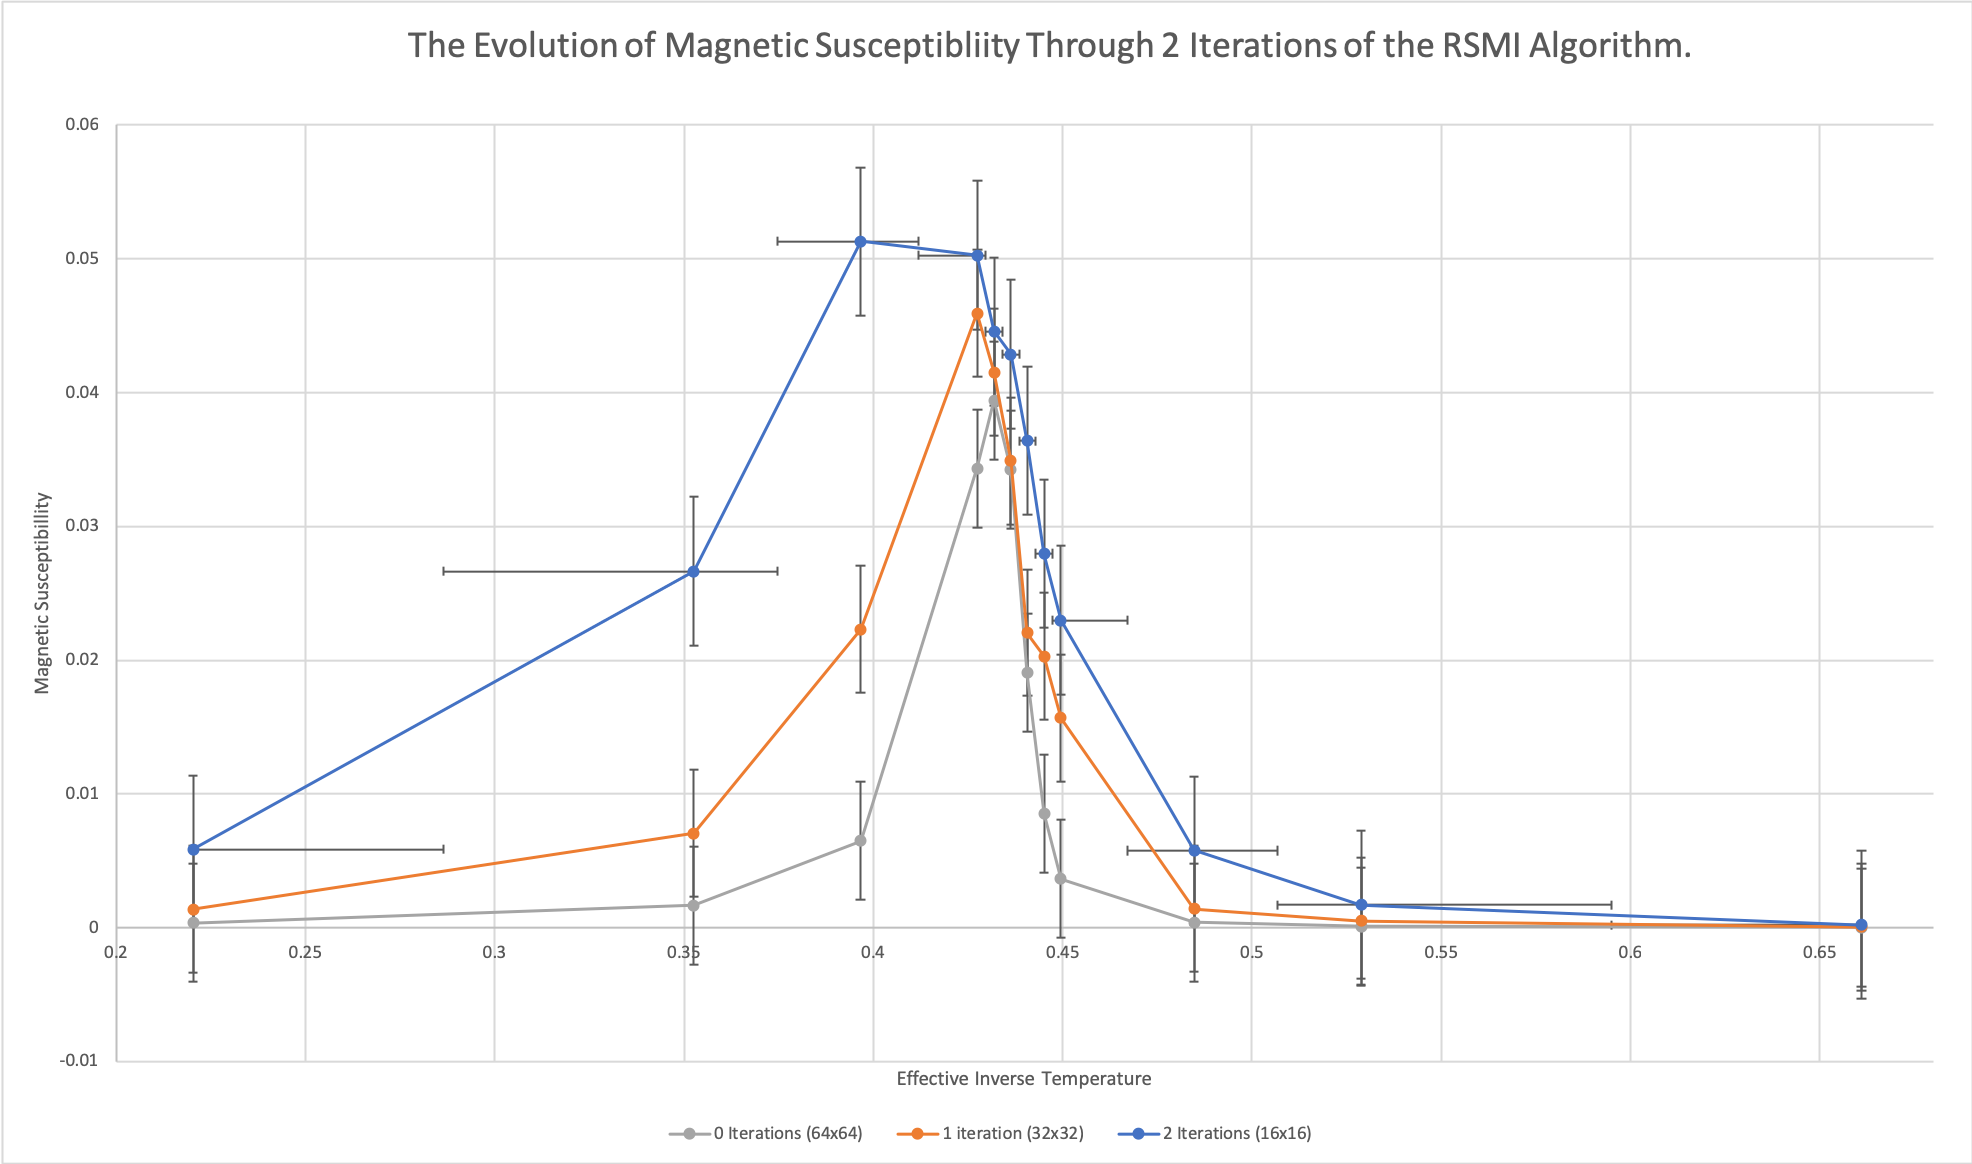
\includegraphics[width=\textwidth]{figures/susceptibility.png}
  \caption{The Magnetic Susceptiblity, $\chi$, at different iterations
    of the RSMI algorithm\label{fig:susceptibility}.}
\end{figure}
